% Senseigigs — system workflow figure, research-paper style.
% Compile: pdflatex -interaction=nonstopmode senseigigs_workflow.tex
%
% SCOPE: the ~0.89 NDCG design only — two stages, retrieval then LambdaMART
% re-ranking. The tier-1 ensemble, cross-encoder and weighted fusion belong to the
% 0.91 variant and are deliberately not drawn.
%
% LAYOUT DISCIPLINE — three defects invisible in source that ruin the render:
%   1. A container tint is OPAQUE (`retC!4` = 4% colour + 96% WHITE, not 4% alpha).
%      Containers are declared after their contents (their `fit=` list needs those
%      nodes), so they paint over every pill and cell. They MUST sit on the
%      background layer — see the pgfonlayer blocks.
%   2. Every box style pins an explicit `text width`; without it a box sizes to its
%      content and sprawls into the next column.
%   3. A fit box must never grow sideways past its own band. Labels that would stick
%      out sit INSIDE, above or below the element they name.
% verify with: python check_layout.py
\documentclass[border=12pt]{standalone}
\usepackage[T1]{fontenc}
\usepackage{tikz}
\usetikzlibrary{arrows.meta, positioning, fit, backgrounds, calc, shapes.geometric}
\usepackage{amssymb}

\definecolor{ioC}{HTML}{2B6CB0}
\definecolor{retC}{HTML}{2F855A}
\definecolor{featC}{HTML}{B7791F}
\definecolor{rankC}{HTML}{C05621}
\definecolor{inkC}{HTML}{2D3748}
\definecolor{dataC}{HTML}{4A5568}
\definecolor{itemC}{HTML}{718096}
\definecolor{goodC}{HTML}{2F855A}

\begin{document}
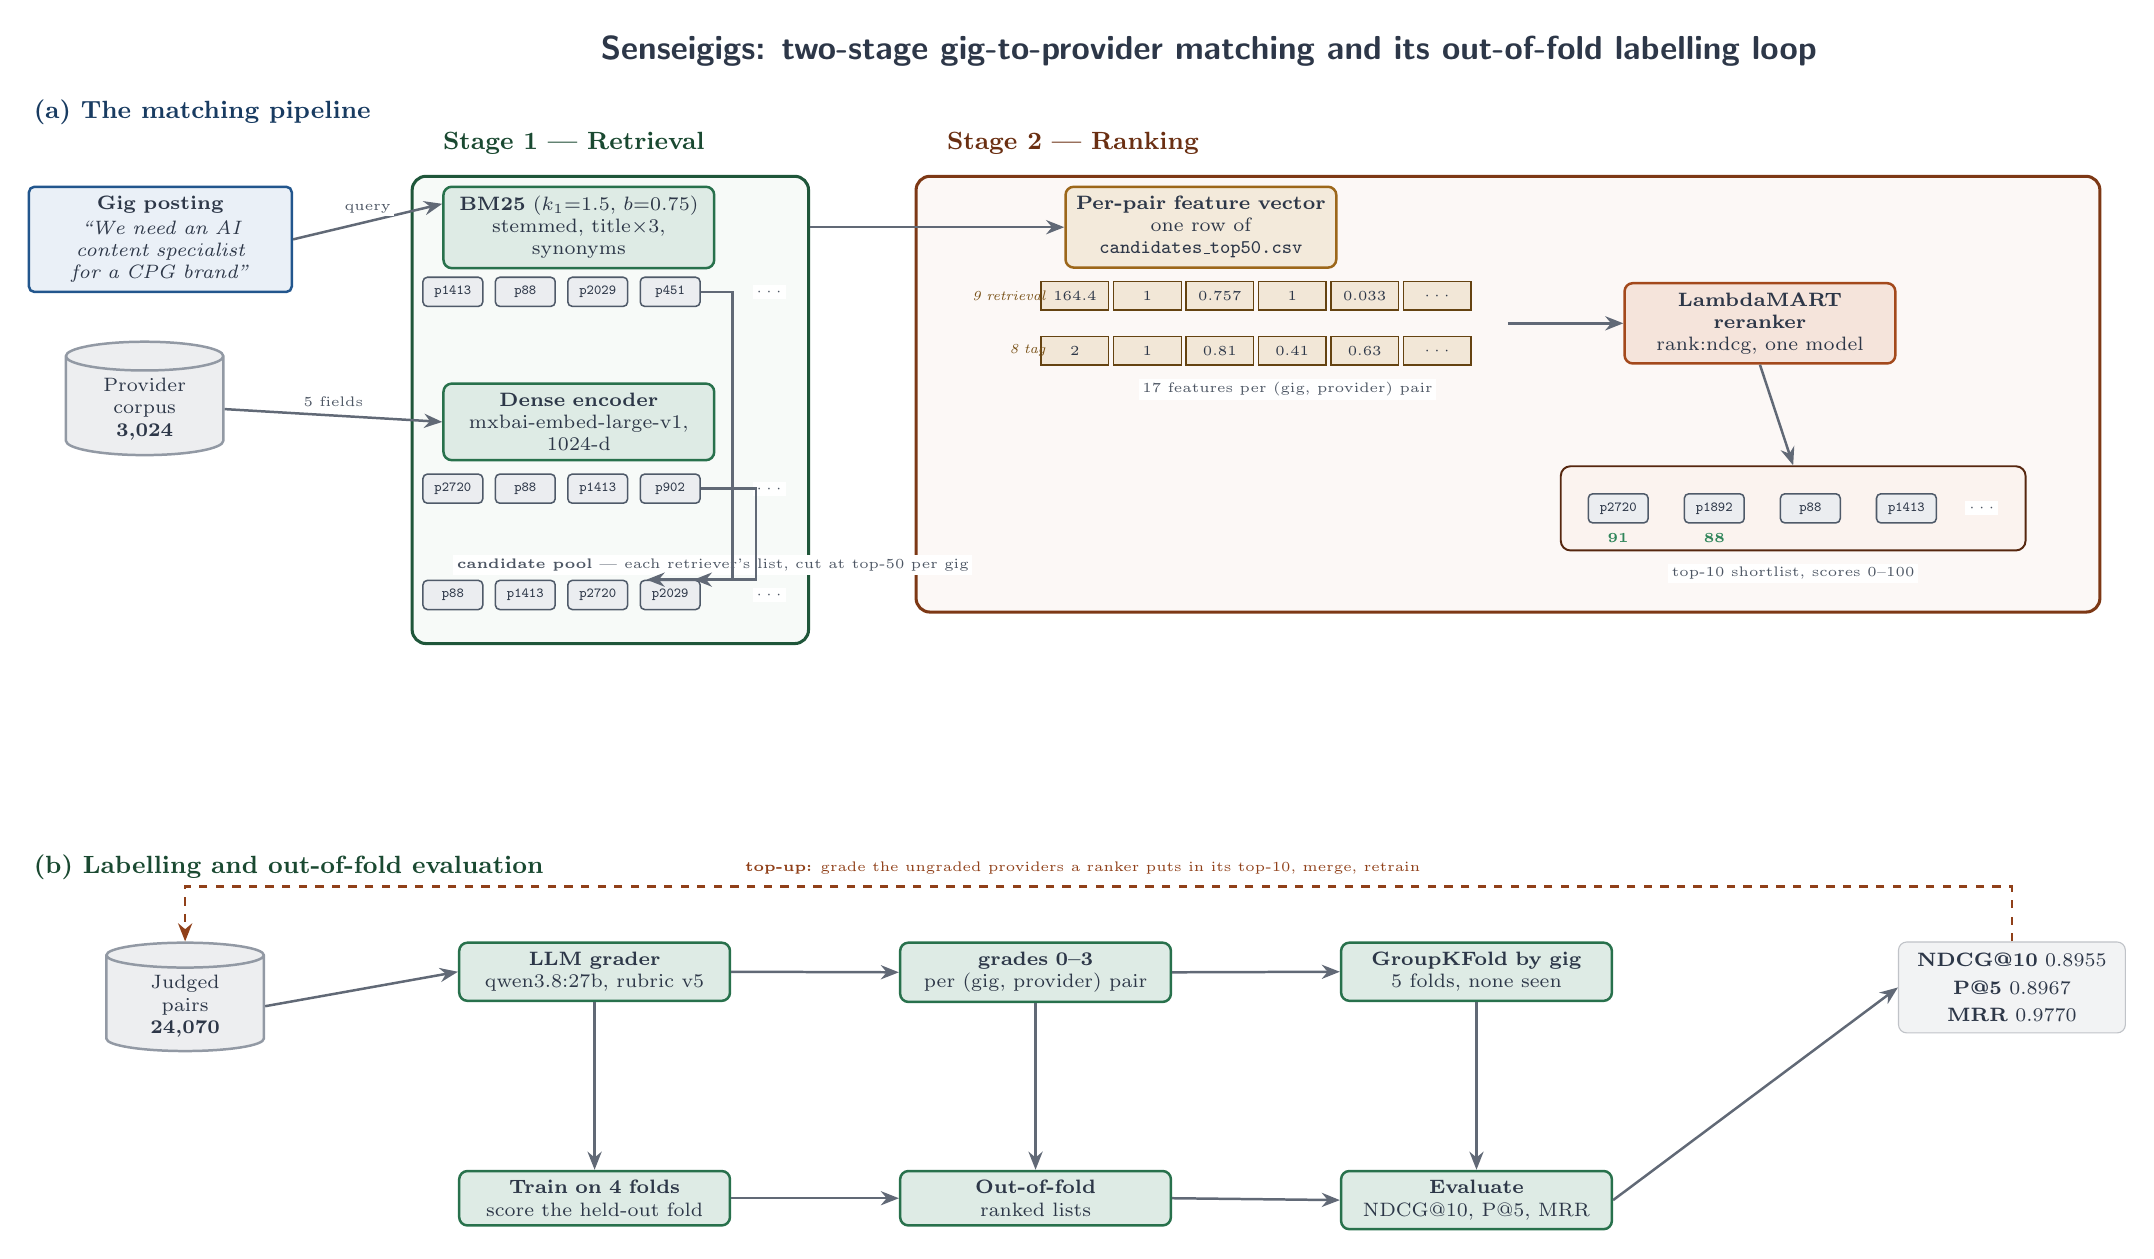
\begin{tikzpicture}[
  font=\sffamily,
  every node/.style={align=center,
    execute at begin node={\hyphenpenalty=10000\exhyphenpenalty=10000}},
  cont/.style={rounded corners=5pt, draw=#1!65!black, fill=#1!4, line width=1.1pt},
  ctitle/.style={font=\small\bfseries, text=#1!55!black},
  mod/.style={rounded corners=3pt, draw=#1!85!black, fill=#1!16, line width=0.9pt,
              inner sep=3.4pt, font=\scriptsize, text=inkC, text width=32mm},
  pill/.style={rounded corners=1.6pt, draw=itemC!70!black, fill=itemC!14, line width=0.55pt,
               inner sep=1.9pt, font=\tiny\ttfamily, text=inkC, minimum height=3.7mm,
               minimum width=7.6mm},
  card/.style={rounded corners=2pt, draw=ioC!80!black, fill=ioC!10, line width=0.9pt,
               inner sep=3.4pt, font=\scriptsize, text=inkC, text width=31mm},
  cyl/.style={cylinder, shape border rotate=90, aspect=0.30, draw=dataC!60, fill=dataC!10,
              line width=0.9pt, inner sep=2.4pt, font=\scriptsize, text=inkC,
              minimum height=12mm, minimum width=20mm},
  fcell/.style={draw=featC!55!black, fill=featC!18, line width=0.5pt, inner sep=1.4pt,
                font=\tiny, text=inkC, minimum height=3.6mm, minimum width=8.6mm},
  flab/.style={font=\tiny\itshape, text=featC!65!black, align=right},
  ar/.style={-{Stealth[length=2.3mm,width=1.8mm]}, line width=0.9pt, draw=inkC!75},
  arl/.style={font=\tiny, text=inkC!85, fill=white, inner sep=1.3pt},
  tb/.style={rounded corners=3pt, draw=inkC!30, fill=inkC!6, inner sep=4pt,
             font=\scriptsize, text=inkC, text width=26mm},
  grp/.style={rounded corners=3.5pt, draw=rankC!45!black, fill=rankC!7,
              line width=0.7pt, inner sep=3.4mm},
]

% ======================= TITLE =======================
\node[font=\sffamily\large\bfseries, text=inkC] at (-8mm,6mm)
  {Senseigigs: two-stage gig-to-provider matching and its out-of-fold labelling loop};

% ============================================================
% PANEL (a) --- the two-stage matching pipeline
% ============================================================
\node[ctitle=ioC, anchor=south west, inner sep=2pt] at (-158mm,-4mm)
  {(a) The matching pipeline};

% ---------- x-band A : inputs ----------
\node[card, anchor=north west] (gig) at (-158mm,-11mm)
  {\textbf{Gig posting}\\[1pt]
   \itshape ``We need an AI\\ content specialist\\ for a CPG brand''};
\node[cyl, anchor=north] (corpus) at ([xshift=-2mm,yshift=-6mm]gig.south)
  {Provider\\corpus\\\textbf{3{,}024}};

% ---------- x-band B : STAGE 1 -- RETRIEVAL ----------
\node[mod=retC, anchor=north] (bm25) at (-88mm,-11mm)
  {\textbf{BM25} ($k_1{=}1.5$, $b{=}0.75$)\\stemmed, title$\times$3, synonyms};
\foreach \t [count=\i] in {p1413,p88,p2029,p451} {%
  \pgfmathsetlengthmacro{\px}{-104mm + (\i-1)*9.2mm}%
  \node[pill] (b25-\i) at (\px,-24.5mm) {\t};}
\node[arl, anchor=west] at (-66mm,-24.5mm) {$\cdots$};

\node[mod=retC, anchor=north] (dense) at (-88mm,-36mm)
  {\textbf{Dense encoder}\\mxbai-embed-large-v1, 1024-d};
\foreach \t [count=\i] in {p2720,p88,p1413,p902} {%
  \pgfmathsetlengthmacro{\px}{-104mm + (\i-1)*9.2mm}%
  \node[pill] (dn-\i) at (\px,-49.5mm) {\t};}
\node[arl, anchor=west] at (-66mm,-49.5mm) {$\cdots$};

% the pooled candidates, with the label INSIDE the container, above the row
\foreach \t [count=\i] in {p88,p1413,p2720,p2029} {%
  \pgfmathsetlengthmacro{\px}{-104mm + (\i-1)*9.2mm}%
  \node[pill] (pool-\i) at (\px,-63mm) {\t};}
\node[arl, anchor=west] at (-66mm,-63mm) {$\cdots$};
\node[arl, anchor=south west] at (-104mm,-60.5mm)
  {\textbf{candidate pool} --- each retriever's list, cut at top-50 per gig};

\coordinate (s1bl) at (-108mm,-68mm);
\coordinate (s1br) at (-60mm,-68mm);
\coordinate (s1tr) at (-60mm,-13mm);
\begin{pgfonlayer}{background}
  \node[cont=retC, fit=(bm25)(b25-1)(b25-4)(dense)(dn-1)(dn-4)(pool-1)(pool-4)
        (s1bl)(s1br)(s1tr)] (S1) {};
\end{pgfonlayer}
\node[ctitle=retC, anchor=south west, inner sep=3pt] at ([xshift=3mm,yshift=1.5mm]S1.north west)
  {Stage 1 --- Retrieval};

% ---------- x-band C : STAGE 2 -- RANKING ----------
\node[mod=featC, anchor=north] (fx) at (-9mm,-11mm)
  {\textbf{Per-pair feature vector}\\one row of \texttt{candidates\_top50.csv}};

% 2 rows: 9 retrieval features, then 8 tag features. Five shown, then an ellipsis.
\foreach \v [count=\i] in {164.4,1,0.757,1,0.033} {%
  \pgfmathsetlengthmacro{\px}{-25mm + (\i-1)*9.2mm}%
  \node[fcell] (fa-\i) at (\px,-25mm) {\v};}
\node[fcell] (fa-6) at (-25mm+5*9.2mm,-25mm) {$\cdots$};
\node[flab, anchor=east] at (-27.5mm,-25mm) {9 retrieval};
\foreach \v [count=\i] in {2,1,0.81,0.41,0.63} {%
  \pgfmathsetlengthmacro{\px}{-25mm + (\i-1)*9.2mm}%
  \node[fcell] (fb-\i) at (\px,-32mm) {\v};}
\node[fcell] (fb-6) at (-25mm+5*9.2mm,-32mm) {$\cdots$};
\node[flab, anchor=east] at (-27.5mm,-32mm) {8 tag};
\node[arl, anchor=north] at (2mm,-35.5mm) {17 features per (gig, provider) pair};

% the model sits to the RIGHT of the grid, vertically centred on it
\node[mod=rankC] (mu) at (62mm,-28.5mm)
  {\textbf{LambdaMART reranker}\\rank:ndcg, one model};
\draw[ar] (30mm,-28.5mm) -- (mu.west);

\foreach \t [count=\i] in {p2720,p1892,p88,p1413} {%
  \pgfmathsetlengthmacro{\px}{44mm + (\i-1)*12.2mm}%
  \node[pill] (out-\i) at (\px,-52mm) {\t};}
\node[arl, anchor=west] (outell) at (88mm,-52mm) {$\cdots$};
\node[goodC, font=\tiny\bfseries, anchor=north] at (out-1.south) {91};
\node[goodC, font=\tiny\bfseries, anchor=north] at (out-2.south) {88};

\coordinate (s2bl) at (-44mm,-64mm);
\coordinate (s2r)  at (104mm,-64mm);
\coordinate (s2tr) at (104mm,-13mm);
\begin{pgfonlayer}{background}
  \node[cont=rankC, fit=(fx)(fa-1)(fa-6)(fb-1)(fb-6)(mu)(out-1)(out-4)
        (s2bl)(s2r)(s2tr)] (S2) {};
\end{pgfonlayer}
\node[ctitle=rankC, anchor=south west, inner sep=3pt] at ([xshift=3mm,yshift=1.5mm]S2.north west)
  {Stage 2 --- Ranking};
\begin{pgfonlayer}{background}
  \node[grp, fit=(out-1)(out-4)(outell)] (outgrp) {};
\end{pgfonlayer}
\node[arl, anchor=north] at ([yshift=-1.5mm]outgrp.south)
  {top-10 shortlist, scores 0--100};


% ============================================================
% PANEL (b) --- labelling + out-of-fold loop
% ============================================================
\node[ctitle=goodC, anchor=south west, inner sep=2pt] at (-158mm,-100mm)
  {(b) Labelling and out-of-fold evaluation};

\node[cyl, anchor=north] (labels) at (-138mm,-107mm) {Judged\\pairs\\\textbf{24{,}070}};
\node[mod=goodC, anchor=north] (grader) at (-86mm,-107mm) {\textbf{LLM grader}\\qwen3.8:27b, rubric v5};
\node[mod=goodC, anchor=north] (grades) at (-30mm,-107mm) {\textbf{grades 0--3}\\per (gig, provider) pair};
\node[mod=goodC, anchor=north] (folds)  at (26mm,-107mm) {\textbf{GroupKFold by gig}\\5 folds, none seen};
\node[mod=goodC, anchor=north] (train)  at (-86mm,-136mm) {\textbf{Train on 4 folds}\\score the held-out fold};
\node[mod=goodC, anchor=north] (oof)    at (-30mm,-136mm) {\textbf{Out-of-fold}\\ranked lists};
\node[mod=goodC, anchor=north] (eval)   at (26mm,-136mm) {\textbf{Evaluate}\\NDCG@10, P@5, MRR};
\node[tb, anchor=north] (metrics) at (94mm,-107mm)
  {\textbf{NDCG@10} 0.8955\\[2pt]\textbf{P@5} 0.8967\\[2pt]\textbf{MRR} 0.9770};

% ---------- flows, panel (a) ----------
\draw[ar] (gig.east)    -- node[arl, midway, above, yshift=0.5mm] {query} ([yshift=3mm]bm25.west);
\draw[ar] (corpus.east) -- node[arl, midway, above, yshift=0.5mm] {5 fields} (dense.west);
% merge the CANDIDATE ROWS (not the model boxes) into the pool
\draw[ar] (b25-4.east) -- ++(4mm,0) |- ([xshift=-3mm]pool-4.north);
\draw[ar] (dn-4.east)  -- ++(7mm,0) |- ([xshift=3mm]pool-4.north);
% stage 1 -> stage 2, entering the feature box
\draw[ar] (S1.east |- fx.west) -- (fx.west);
% model -> shortlist
\draw[ar] (mu.south) -- (outgrp.north);

% ---------- flows, panel (b) ----------
\draw[ar] (labels.east)  -- (grader.west);
\draw[ar] (grader.east)  -- (grades.west);
\draw[ar] (grades.east)  -- (folds.west);
\draw[ar] (grader.south) -- (train.north);
\draw[ar] (grades.south) -- (oof.north);
\draw[ar] (folds.south)  -- (eval.north);
\draw[ar] (train.east)   -- (oof.west);
\draw[ar] (oof.east)     -- (eval.west);
\draw[ar] (eval.east)    -- (metrics.west);

% the top-up loop
\draw[ar, draw=rankC!75!black, dashed]
  (metrics.north) |- ([yshift=7mm]labels.north) -- (labels.north);
\node[arl, text=rankC!75!black, anchor=south] at (-24mm,-99mm)
  {\textbf{top-up:} grade the ungraded providers a ranker puts in its top-10, merge, retrain};

\end{tikzpicture}
\end{document}
